\documentclass{article}
\usepackage[utf8]{inputenc}
\usepackage{tikz}
\usepackage{circuitikz}
\usepackage{geometry}
\geometry{margin=1in}
\usepackage{listings}
\usepackage{xcolor}
\geometry{margin=1in}
\title{Servo Motor Documentation - Raspberry Pi 5 Integration}
\author{El Mehdi Adnani Kadmiri}
\date{July 21, 2025}

\lstset{
	basicstyle=\ttfamily\small,
	keywordstyle=\color{blue},
	commentstyle=\color{gray},
	stringstyle=\color{teal},
	breaklines=true,
	frame=single,
	postbreak=\mbox{\textcolor{red}{$\hookrightarrow$}\space}
}

	\begin{document}
		
	\maketitle
	
		\section{Description}
	\textbf{Servo motors}
	(or “servo”) is an electromechanical device used to precisely control the angular position, speed, or torque of a mechanism. It typically consists of a motor (often an electric motor), a position sensor, and a control circuit, all housed in one enclosure.
	The servomotor operates in a closed loop: it continuously compares the current position to the desired position, then adjust motor movement to eliminate any deviation. This is called a position-controlled system.
	
	Servomotors are used in many fields, including robotics, automatic control systems, and industrial machines to perform precise and controlled movements. They are particularly valued for their accuracy, responsiveness, and ability to maintain a stable position even in the presence of external disturbances.

	\section{Applications}
	\begin{itemize}
		\item \textbf{CNC Machines:} Computer numerical control (CNC) machines use servo motors to precisely control the cutting tools and workpieces. For complex item manufacturing, such as in metalworking and woodworking, servo motors' precise control over a wide range of speeds and locations is crucial.
		\item \textbf{Robotics:} Industrial robots, which perform a variety of tasks like welding, painting, and picking and packing, frequently run on servo motors. Robots can carry out intricate movement sequences thanks to the motors' accuracy and reactivity, which raises the degree of automation and increases the flexibility of production processes.
		\item \textbf{	Material Handling Systems:} Servo motors make it easier for commodities to move through conveyors, sorters, and automated storage and retrieval systems (AS/RS) in logistics and warehousing. Their precise positional and speed control maximizes material flow, reducing handling times and boosting output.
	\end{itemize}
	
	\section{Working Principle}
		Servo motors are controlled using \textbf{Pulse Width Modulation (PWM) signals}. A PWM signal is a series of pulses where the width of the "on" pulse determines the desired position of the servo motor's shaft. The servo motor's internal circuitry interprets the pulse width and adjusts the motor's position accordingly.
		\begin{itemize}
			\item A 1 ms pulse = 0° (minimum position)
			\item A 1.5 ms pulse = 90° (center position)
			\item A 2 ms pulse = 180° (maximum position)
		\end{itemize}
		PWM signals are repeated approximately every 20 ms (50 Hz). The duration of the pulse within that time frame determines the servo position.
		
	
	\section{Wiring Diagram}
	\begin{center}
		\begin{tabular}{|c|c|c|}
			\hline
			\textbf{Servo Motor Pin} & \textbf{Raspberry Pi Pin} & \textbf{Function} \\
			\hline
			VCC & 4.8 - 6 V  & Power \\
			GND & GND & Ground \\
			OUT & GPIO17 (or any output) & signal \\
			\hline
		\end{tabular}
	\end{center}
	
	\begin{center}
		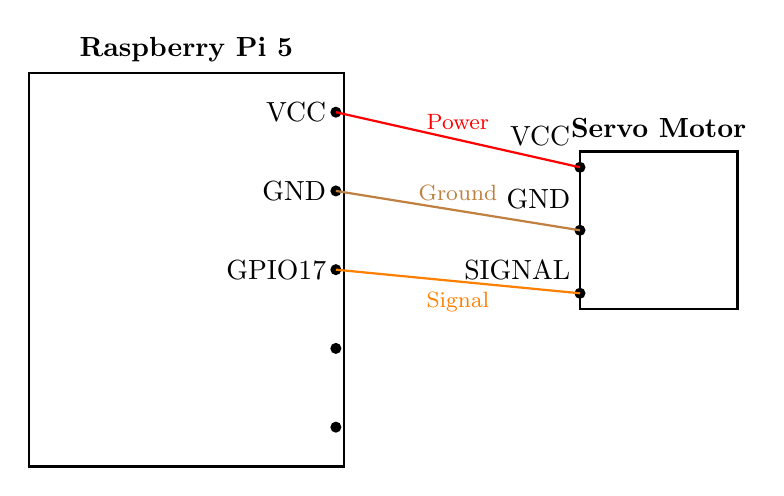
\begin{tikzpicture}
			
			% Raspberry Pi rectangle
			\draw[thick] (0,0) rectangle (4,5);
			\node at (2,5.3) {\textbf{Raspberry Pi 5}};
			\node[anchor=east] at (3.9,4.5) {VCC};
			\node[anchor=east] at (3.9,3.5) {GND};
			\node[anchor=east] at (3.9,2.5) {GPIO17};
			% GPIO pins
			
			\fill (3.9,4.5) circle (2pt); % 3.3V
			\fill (3.9,3.5) circle (2pt); % GND
			\fill (3.9,2.5) circle (2pt);
			\fill (3.9,1.5) circle (2pt);
			\fill (3.9,0.5) circle (2pt);
			% GPIO17
				% Servomotor rectangle
			\draw[thick] (7,2) rectangle (9,4);
			\node at (8,4.3) {\textbf{Servo Motor}};
			% Sensor pins
			\node[anchor=east] at (7,4.2) {VCC};
			\node[anchor=east] at (7,3.4) {GND};
			\node[anchor=east] at (7,2.5) {SIGNAL};
			% Dots for sensor pins
			\fill (7,3.8) circle (2pt); % VCC
			\fill (7,3.0) circle (2pt); % GND
			\fill (7,2.2) circle (2pt); % OUT
			
			% Connecting lines
			\draw[red, thick] (3.9,4.5) -- (7,3.8) node[midway, above] {\footnotesize Power};
			\draw[brown, thick] (3.9,3.5) -- (7,3.0) node[midway, above] {\footnotesize Ground};
			\draw[orange, thick] (3.9,2.5) -- (7,2.2) node[midway, below] {\footnotesize Signal};
		\end{tikzpicture}
	\end{center}
	\section{Libraries Used}
	\subsection*{Python: RPi.GPIO}
	These libraries allow for PWM signal generation using GPIO pins.
	\begin{itemize}
		\item \textbf{RPi.GPIO:}
		\begin{itemize}
			\item Import: \texttt{import RPi.GPIO as GPIO}
			\item Setup: \texttt{GPIO.setmode(GPIO.BCM)}
			\item PWM Start: \texttt{GPIO.PWM(18, 50)}
		\end{itemize}
		
	\end{itemize}
	
	\subsection*{C: pigpio Library/SoftPWM}
	\texttt{pigpio} offers precise PWM control in C.
	\begin{itemize}
		\item Include: \texttt{\#include <pigpio.h>}
		\item Init: \texttt{gpioInitialise();}
		\item PWM: \texttt{gpioServo(18, 1500);}
	\end{itemize}
	\texttt{softPwm} is an extension of the WiringPi library that allows software PWM generation on any GPIO pin. It is particularly useful for controlling devices like servo motors, which require precise PWM signals for angle positioning.
	
	\begin{itemize}
		\item Setup: \texttt{softPwmCreate(pin, initialValue, range)}
		\item Change PWM value: \texttt{softPwmWrite(pin, value)}
		\item Example range: 0–100 (interpreted as 0\% to 100\% duty cycle)
	\end{itemize}

	\section{Python Example}
	\begin{lstlisting}[language=Python]
		import RPi.GPIO as GPIO
		import time
		
		SERVO_PIN = 18
		
		GPIO.setmode(GPIO.BCM)
		GPIO.setup(SERVO_PIN, GPIO.OUT)
		
		pwm = GPIO.PWM(SERVO_PIN, 50)  # 50 Hz
		pwm.start(0)
		
		try:
		while True:
		# Rotate to 0
		pwm.ChangeDutyCycle(2.5)
		time.sleep(1)
		
		# Rotate to 90
		pwm.ChangeDutyCycle(7.5)
		time.sleep(1)
		
		# Rotate to 180
		pwm.ChangeDutyCycle(12.5)
		time.sleep(1)
		
		except KeyboardInterrupt:
		pwm.stop()
		GPIO.cleanup()
	\end{lstlisting}
	
	\section{C Example}
	\begin{lstlisting}[language=C]
		#include <wiringPi.h>
		#include <softPwm.h>
		#include <stdio.h>
		
		#define SERVO_PIN 1 // wiringPi pin 1 = BCM 18
		
		int main(void) {
			wiringPiSetup();
			softPwmCreate(SERVO_PIN, 0, 200); // Range 0-200
			
			while (1) {
				// Rotate to 0
				softPwmWrite(SERVO_PIN, 5);
				delay(1000);
				
				// Rotate to 90
				softPwmWrite(SERVO_PIN, 15);
				delay(1000);
				
				// Rotate to 180
				softPwmWrite(SERVO_PIN, 25);
				delay(1000);
			}
			
			return 0;
		}
	\end{lstlisting}
	
	\section{Conclusion}
	The servo motor enables precise angular motion control and is easily controlled by PWM signals on the Raspberry Pi. Both Python and C implementations demonstrate how simple it is to move the motor between defined positions for practical applications like robotics or camera panning.
	
	
	
 
\end{document}
	